En este capítulo se expondrá la metodología a seguir en el proyecto, así como el planeamiento de las actividades que se llevarán a cabo para completarlo. 

\section{Ciencia del diseño}
Este proyecto se desarrollará bajo la metodología de la ciencia del diseño. En esta metodología se busca diseñar e investigar artefactos en un contexto específico~\cite{wieringa_design_2014}. Dentro de esta metodología los artefactos son cualquier cosa que es diseñada por la persona investigadora, desde programas de software hasta técnicas. Por otra parte, el contexto es todo aquello que no puede ser diseñado por la persona investigadora, como el hardware en el que se ejecutará el programa o las restricciones de presupuesto.
En la~\cref{fig:artifact} podemos observar la relación entre el artefacto y el contexto en nuestra investigación. El artefacto será una simulación sismológica que hace uso de la visualización y análisis in-situ que se desarrollará, mientras que el contexto incluye el hardware que tenemos disponible para ejecutar las simulaciones, los datos que tenemos disponibles, los contactos que se cuentan con sismólogos corresponde a las técnicas computacionales aplicadas a la sismología. Es importante siempre tener en cuenta el contexto mientras se realiza el desarrollo de la simulación ya que es la interacción entre ambos lo que llevará a la resolución del problema.
\begin{figure}
  \centering
  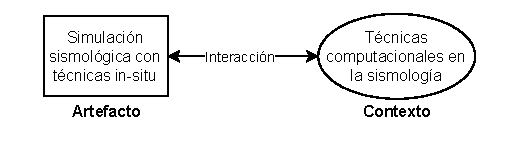
\includegraphics[width=0.9\textwidth]{artifact_context}
  \caption{Tema de investigación}
  \label{fig:artifact}
\end{figure}

\section{Actividades a realizar}
\label{sec:activities}

El marco de trabajo que se utiliza en la ciencia del diseño se presenta en la~\cref{fig:framework}. El contexto social se refiere a aquellas personas que impactan y son impactadas por nuestra investigación. En nuestro caso las personas interesadas son investigadores en sismología, los desarrolladores de bibliotecas in-situ y los desarrolladores de la simulación sismológica SeisSol. El contexto del conocimiento se refiere a las áreas del saber que impactan y son impactadas por el proyecto. En nuestro caso estas incluyen la sismología, las técnicas de análisis y visualización in-situ y la computación de alto rendimiento.

En la ciencia del diseño, un problema de investigación se divide en problemas de diseño y preguntas de conocimiento. Los primeros se resuelven con ciclos de diseño y los segundos con ciclos empíricos. En nuestro proyecto identificamos las siguientes partes:

\begin{itemize}
    \item Pregunta de conocimiento 1 (PC1): ¿Cuáles técnicas in-situ se utilizan en otros dominios de la ciencia a parte de la sismología?
    \item Problema de diseño (PD): La extensión de una simulación sísmica numérica para que utilice el análisis y la visualización in-situ.
    \item Pregunta de conocimiento 2 (PC2): ¿Qué tan efectiva es la herramienta desarrollada en términos de ciencia y rendimiento computacional?
\end{itemize}
Cada una de estas partes corresponde con un objetivo específico del proyecto los cuales reproducimos a continuación:
\begin{enumerate}
  \item Caracterizar simulaciones en otros dominios que hayan incorporado el análisis in-situ. % Explicar que esto terminará en un artículo.
  \item Extender una simulación sísmica numérica para que utilice el análisis y la visualización in-situ. % Explicar que esto incluye el diseño y mejora del rendimiento del programa.
  \item Estudiar el rendimiento y validar la utilidad de la simulación extendida. % Explicar que esto incluirá el criterio de expertos en el área.
\end{enumerate}

El ciclo empírico (CE1) para responder la PC1 tendrá como objetivo el caracterizar simulaciones en otros dominios que hayan incorporado el análisis in-situ. Para realizar esto se llevará a cabo una revisión sistemática de literatura utilizando los parámetros definidos en las recomendaciones PRISMA 2020~\cite{Page2021}. 

% Las actividades relacionadas a este ciclo son las siguientes:
% \newcounter{tasks}
% \begin{enumerate}
%     \item Definir los parámetros de la revisión: Esta actividad incluye la delimitación de la búsqueda, la creación del protocolo de revisión, la selección de bases de datos y las hileras de búsqueda y la definición de los criterios de inclusión y exclusión.
%     \item Llevar a cabo la revisión: Aquí se llevará a cabo la búsqueda de los artículos científicos, así como la aplicación de los criterios de inclusión y exclusión, y la extracción de datos con el protocolo de revisión.
%     \item Análisis de datos: Se analizarán los datos que extrajeron de la revisión y se llegará a conclusiones que se podrán utilizar para informar el desarrollo del proyecto actual.
%     \setcounter{tasks}{\value{enumi}}
% \end{enumerate}
En el ciclo de diseño (CD) para resolver el PD se extenderá la simulación SeisSol para que haga uso de técnicas de análisis y visualización in-situ. Para lograr esto se hará uso del conocimiento obtenido en el CE1 para informar el diseño de la solución, así como el análisis de la base de código y consultas a los autores de la simulación y las bibliotecas de análisis y visualización in-situ. 
Se llevarán a cabo consultas con investigadores del Observatorio vulcanológico y sismológico de Costa Rica (OVSICORI) para definir escenarios de simulación que servirán para validar el funcionamiento de la simulación antes y después de los cambios a realizar, así como su rendimiento computacional. Será necesario entonces ejecutar la simulación sin modificaciones para tener un entendimiento de cómo se comporta esta de manera inicial. Estas pruebas se llevarán a cabo en la supercomputadora Polaris del laboratorio nacional Argonne (ANL) en EEUU. Con esta base, se llevarán a cabo las modificaciones al código, esto se realizará en la sección del programa que realiza el ciclo principal de la simulación utilizando la biblioteca Ascent. Se mantendrá comunicación con la comunidad de desarrolladores de SeisSol para que estén al tanto de estas modificaciones en caso de que se considere que sea provechozo mezclarlas al tronco principal del repositorio. Una vez hechas las modificaciones se llevaran a cabo las pruebas con los escenarios escogido anteriormente, mientras se atienden los problemas que se encuentren gracias a la ejecución de los casos.

Finalmente, en el segundo ciclo empírico (CE2) se responderá la PC2. Se realizarán validaciones de los resultados obtenidos con sismólogos. También se realizarán pruebas de rendimiento computacional, escalamiento fuerte y débil, las cuales servirán para conocer los límites de la herramienta, así como encontrar el overhead de las modificaciones realizadas al código. Las validaciones con los expertos se realizarán mediante entrevistas en donde se evaluará la calidad de la simulación, así como la utilidad percibida de la misma. En cuanto a las pruebas de rendimiento computacional, se 

De forma transversal se estará documentando el avance del proyecto.

\begin{figure}[h]
    \centering
    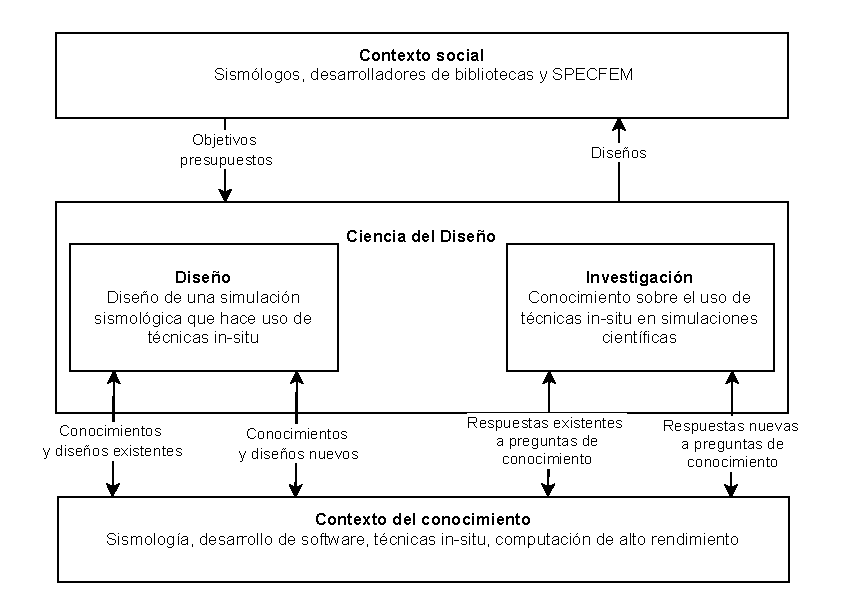
\includegraphics{framework}
    \caption{Marco de trabajo en el que se desarrolla la investigación}
    \label{fig:framework}
\end{figure}

\section{Cronograma}
Las actividades definidas en el~\cref{sec:activities} se llevarán a cabo según el cronograma que se encuentra en la~\cref{fig:chronogram}.

\begin{figure}
    \centering
    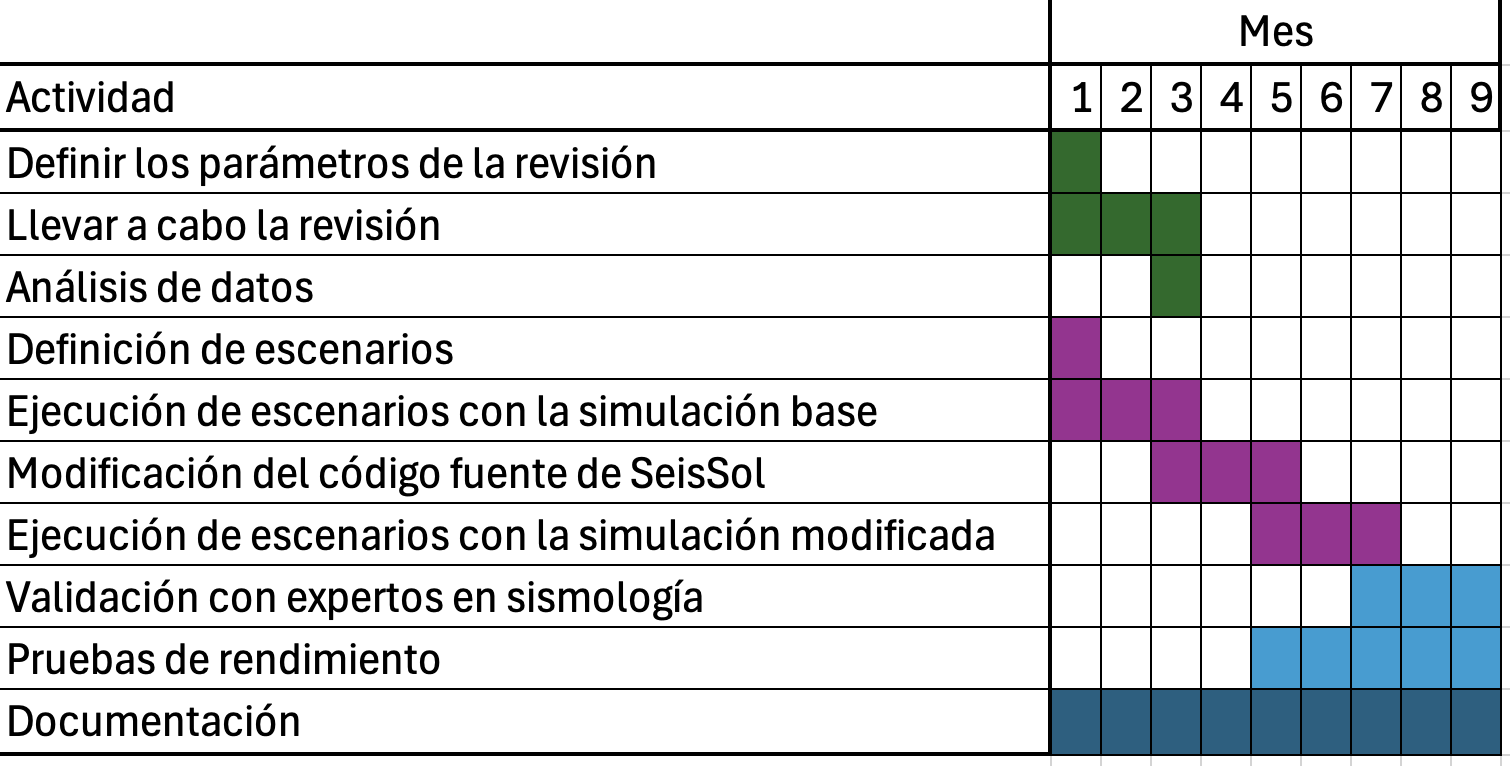
\includegraphics[width=0.7\textwidth]{chronogram}
    \caption{Cronograma tentativo para el desarrollo del proyecto.}
    \label{fig:chronogram}
\end{figure}